% !TEX program = xelatex
% !TEX program = xelatex
% LAB1 도입부와 레거시 01 실습. 나머지 본문은 이후 이어 작성한다.
% 이 폴더에서 xelatex -interaction=nonstopmode -halt-on-error로 두 번 빌드한다.
% 디자인 원본: ../../templates/weekly_presentation_template_4x3.tex
% 구성 기준: ../../../daily_goal/GOAL0910.md
\documentclass[aspectratio=43,11pt,t]{beamer}

\usepackage{fontspec}
\usepackage{kotex}
\usepackage{graphicx}
\usepackage{tikz}
\usepackage{etoolbox}
\setmainfont{D2Coding-Regular.ttf}[Path=../../assets/fonts/,BoldFont={D2Coding-Bold.ttf}]
\setmainhangulfont{D2Coding-Regular.ttf}[Path=../../assets/fonts/,BoldFont={D2Coding-Bold.ttf}]
\setsansfont{D2Coding-Regular.ttf}[Path=../../assets/fonts/,BoldFont={D2Coding-Bold.ttf}]
\setsanshangulfont{D2Coding-Regular.ttf}[Path=../../assets/fonts/,BoldFont={D2Coding-Bold.ttf}]
\setmonofont{D2Coding-Regular.ttf}[Path=../../assets/fonts/,BoldFont={D2Coding-Bold.ttf}]

\definecolor{UOSBlue}{HTML}{005EB8}
\definecolor{TextGray}{HTML}{303030}
\setbeamertemplate{navigation symbols}{}
\setbeamercolor{normal text}{fg=TextGray,bg=white}
\setbeamercolor{frametitle}{fg=UOSBlue,bg=white}
\setbeamercolor{title}{fg=white}
\setbeamercolor{structure}{fg=UOSBlue}
\setbeamertemplate{itemize item}{\color{UOSBlue}\small$\bullet$}
\setbeamertemplate{frametitle}{%
  \vspace{0.55cm}\hspace{0.48cm}\insertframetitle\par\vspace{0.12cm}}
\setbeamerfont{frametitle}{series=\bfseries,size=\LARGE}
\setbeamertemplate{footline}{%
  \begin{tikzpicture}[remember picture,overlay]
    \node[anchor=south,inner sep=0pt] at ([yshift=0.52cm]current page.south)
      {
\includegraphics[width=2.64cm,trim=58bp 385bp 58bp 385bp,clip]{../../assets/uos-logo-horizontal.png}};
    \node[anchor=west,text=UOSBlue,font=\scriptsize]
      at ([xshift=0.65cm,yshift=0.52cm]current page.south west)
      {\labonehome};
    \node[anchor=east,text=gray,font=\scriptsize]
      at ([xshift=-0.57cm,yshift=0.52cm]current page.south east) {\insertframenumber};
  \end{tikzpicture}%
  \vspace{0.38cm}}

\newcommand{\course}{전자전기컴퓨터설계실험Ⅱ}
\newcommand{\presenter}{이해리}
% 표지 날짜는 수업일이 아니라 자료 작성일이다.
\newcommand{\materialdate}{2026. 09. 10.}
\newcommand{\contentsbutton}{\beamerbutton{\strut\hspace{0.5em}목차\hspace{0.5em}}}
\newcommand{\labonehome}{\hyperlink{lab1-contents}{\contentsbutton}}
\newcommand{\navlink}[2]{\hyperlink{#1}{\textcolor{UOSBlue}{#2}}}
\newcommand{\legacySource}[1]{%
  \begin{tikzpicture}[remember picture,overlay]
    \node[anchor=west,text=gray,font=\tiny]
      at ([xshift=0.65cm,yshift=1.02cm]current page.south west)
      {원본: 논리 게이트 구현, p.#1\quad\hyperlink{legacy-01}{레거시 01}};
  \end{tikzpicture}}
\title{\course\\LAB 1. 조합회로 실습}
\author{\presenter}
\date{\materialdate}
\hypersetup{pdftitle={LAB1 조합회로 실습 — 레거시 01},pdfauthor={이해리}}

\renewcommand{\labonehome}{\hyperlink{legacy-01-contents}{\contentsbutton}}
\renewcommand{\legacySource}[1]{}
\hypersetup{pdftitle={AND·OR·XOR 논리 게이트}}
\providecommand{\terminalbox}[1]{\par\vspace{0.15cm}{\setlength{\fboxsep}{7pt}\colorbox{black}{\parbox{\dimexpr\textwidth-14pt\relax}{\color{white}\ttfamily\fontsize{7}{9}\selectfont #1}}}\par\vspace{0.15cm}}
\begin{document}
\begingroup
\renewcommand{\small}{\fontsize{9}{11}\selectfont}
\begin{frame}{01 · AND·OR·XOR 논리 게이트}\relax
\small
VS Code 사전 시뮬레이션 → 레거시 Vivado → 보드 실험\par\vspace{0.22cm}같은 입력 a, b에 대해 x는 AND, y는 OR, z는 XOR이다.\par\begin{enumerate}\setlength{\itemsep}{0.22cm}
\item 템플릿을 clone하고 이 회로의 workspace를 연다.
\item 예상값을 계산하고 RTL·TB·XDC를 직접 작성해 시뮬레이션한다.
\item Vivado 결과와 실제 보드 동작을 비교한다.
\item 자신의 사진·영상·레포트를 GitHub에 연결한다.
\end{enumerate}
작성일 2026. 09. 10. · 이해리\par
\end{frame}

\begin{frame}[label=legacy-01-contents]{실습 목차}\relax
\small
1부 · VS Code 사전 실습\par\navlink{legacy-01-setup}{새 창·workspace·확장·코드 열기}\par\vspace{0.2cm}
\navlink{legacy-01-sim}{예상값·작업 실행·로그·파형·실험 전 레포트}\par\vspace{0.4cm}
2부 · Vivado 실습\par\navlink{legacy-01-vivado}{프로젝트·소스·top·시뮬레이션·핀·비트스트림}\par\vspace{0.4cm}
3부 · 결과 정리\par\navlink{legacy-01-post}{보드·사진·영상·GitHub·실험 후 레포트}\par\vspace{0.35cm}
\href{04.LAB1_00_CONTENTS.pdf}{전체 목차 PDF 열기}
\end{frame}

\begin{frame}[label=legacy-01-setup]{시뮬레이션 도구 확인}\relax
\small
Git·Python 3.10 이상·VS Code·Icarus Verilog를 설치한다. Windows PowerShell에서 한 줄씩 확인한다.\par\terminalbox{git --version\\python --version\\iverilog -V\\vvp -V}
설치·PATH 변경 후 VS Code를 다시 연다. Linux·macOS·WSL은 python 대신 python3를 사용한다.\par\href{https://github.com/Glaysia/fpga-lab-template/tree/v2.0.0}{설치와 빈 템플릿 안내}
\end{frame}

\begin{frame}{v2.0.0 템플릿을 새 이름으로 clone}\relax
\small
아래는 Windows PowerShell 명령이다. 줄 끝 문자는 다음 줄로 명령을 이어 준다.\par\terminalbox{git clone --branch v2.0.0 `\\  https://github.com/Glaysia/fpga-lab-template.git `\\  lab1\_legacy\_01\_logic\_gates\\cd lab1\_legacy\_01\_logic\_gates\\git switch -c main\\code LAB1.code-workspace}
회로마다 마지막 폴더 이름을 바꾼다. 시작 파일은 주석뿐이며 코드 이미지를 보며 직접 작성한다.\par\href{https://github.com/Glaysia/fpga-lab-template/tree/v2.0.0}{고정된 수업 버전 v2.0.0}
\end{frame}

\begin{frame}{File → New Window}\relax
\small
VS Code 상단 File → New Window. Ctrl+Shift+N도 같은 동작이다.\par\par\vspace{0.18cm}{\centering\includegraphics[width=\textwidth,height=1.6cm,keepaspectratio,trim=27.75bp 522bp 652.5bp 21bp,clip]{assets/modern-01/01-file-menu.png}\par}\vspace{0.16cm}
새 창의 File → Open Workspace from File...을 누른다.\par\par\vspace{0.18cm}{\centering\includegraphics[width=\textwidth,height=1.6cm,keepaspectratio,trim=27.75bp 439.5bp 652.5bp 105bp,clip]{assets/modern-01/01-file-menu.png}\par}\vspace{0.16cm}

\end{frame}

\begin{frame}{프로젝트 하나의 workspace 열기}\relax
\small
\begin{enumerate}\setlength{\itemsep}{0.22cm}
\item 방금 clone한 lab1\_legacy\_01\_logic\_gates 폴더를 연다.
\item LAB1.code-workspace를 선택하고 Open. 모든 실습의 workspace 파일명은 같다.
\item Explorer에 PROJECT 하나와 src·sim·constraints·tools 폴더가 보이는지 확인한다.
\item src/design.v·sim/tb\_design.v·constraints/pins.xdc는 아직 주석뿐이다.
\item simulation.json은 실행할 RTL·TB 파일과 TB top을 지정하는 설정이다.
\end{enumerate}

\end{frame}

\begin{frame}{추천 확장 설치}\relax
\small
\begin{enumerate}\setlength{\itemsep}{0.22cm}
\item 왼쪽 Extensions 아이콘을 누른다.
\item 검색창에 @recommended를 입력한다.
\item slang의 Install: Verilog/SystemVerilog 편집·진단.
\item VaporView의 Install: VCD 파형 확인.
\item vscode-pdf의 Install: 코드 옆에서 PDF 교안 열기.
\end{enumerate}
WSL 사용자는 WSL 창에서 필요할 경우 Install in WSL을 누른다. 확장 설치와 Python·Icarus 설치는 별개다.\par
\end{frame}

\begin{frame}{src에 RTL 파일 만들기}\relax
\small
\begin{enumerate}\setlength{\itemsep}{0.22cm}
\item Explorer에서 src 왼쪽 화살표를 눌러 펼친다.
\item design.v 우클릭 → Rename → logic\_gate.v 입력.
\item 파일을 두 번 눌러 열고 뒤의 코드 이미지를 보며 전체 코드를 입력한다.
\item 추가 RTL이 있으면 src 우클릭 → New File로 만든다.
\item 전체 RTL 파일 목록은 다음 장의 src 표를 따른다.
\item File → Save All로 모든 파일을 저장한다.
\end{enumerate}
설계 모듈명: logic\_gate. 파일명과 module 이름을 구분한다.\par
\end{frame}

\begin{frame}{sim에 테스트벤치 만들기}\relax
\small
\begin{enumerate}\setlength{\itemsep}{0.22cm}
\item sim을 펼치고 tb\_design.v 우클릭 → Rename.
\item 새 파일명: tb\_logic\_gate\_modern.sv
\item 뒤의 TB 코드 이미지에 있는 선언·DUT 연결·입력 자극·예상값 검사를 직접 작성한다.
\item wave.vcd를 만드는 dumpfile·dumpvars와 종료 조건까지 작성한다.
\item TB 모듈명: tb\_logic\_gate\_modern
\item File → Save All. TB를 합성용 RTL 폴더에 넣지 않는다.
\end{enumerate}

\end{frame}

\begin{frame}{작성할 RTL 파일 목록}\relax
\small
\begin{center}\renewcommand{\arraystretch}{1.45}
\begin{tabular}{l|l}
폴더 & 파일명\\\hline
src & logic\_gate.v\\
\end{tabular}\end{center}
각 파일을 New File로 만들고 코드 이미지의 전체 내용을 작성한다. 파일마다 module 선언과 endmodule을 확인한다.\par
\end{frame}

\begin{frame}{simulation.json을 내 파일에 맞추기}\relax
\small
Explorer에서 simulation.json을 두 번 눌러 연다.\par\vspace{0.22cm}sources 배열: 앞의 모든 RTL 파일명 앞에 src/를 붙여 등록한다.\par\vspace{0.22cm}한 파일 예: "sources": ["src/logic\_gate.v"]\par\vspace{0.22cm}testbench: sim/tb\_logic\_gate\_modern.sv\par\vspace{0.22cm}simulation\_top: tb\_logic\_gate\_modern\par\vspace{0.22cm}sources의 각 경로와 testbench·simulation\_top 값은 큰따옴표로 감싼다. 여러 경로는 쉼표로 구분한다.\par\vspace{0.22cm}파일명·확장자·괄호·쉼표를 확인하고 Save All.\par
\end{frame}

\begin{frame}{VS Code 실습은 대응 최신판을 재사용}\relax
\small
이 PDF의 사전 실습은 01번 최신판과 같은 RTL·자기검사 TB·실행 방법이다.\par\vspace{0.22cm}실습 폴더는 이번 레거시용 이름으로 만들되, 같은 코드 이미지를 보고 직접 작성한다.\par\vspace{0.22cm}VS Code의 PASS·파형·실험 전 레포트 뒤에 이 PDF의 원본 Vivado 강의자료를 진행한다.\par\vspace{0.22cm}원본 testbench.v는 자극 순서·시간이 다를 수 있다. 동일 결과 비교에는 앞에서 작성한 자기검사 TB를 등록한다.\par\href{04.LAB1_01_LOGIC_GATES_VIVADO.pdf}{01번 VS Code 상세 실습 열기}
\end{frame}

\begin{frame}[label=legacy-01-sim]{입출력과 동작 규칙}\relax
\small
입력 a, b / 출력 x, y, z\par\vspace{0.22cm}같은 입력 a, b에 대해 x는 AND, y는 OR, z는 XOR이다.\par\vspace{0.22cm}KEY1=a, KEY2=b. LED1=x, LED2=y, LED3=z.\par
\end{frame}

\begin{frame}{실행 전에 예상값 작성}\relax
\small
\begin{center}\renewcommand{\arraystretch}{1.45}
\begin{tabular}{l|l}
입력 또는 조건 & 예상 결과\\\hline
00 & 000\\
01 & 011\\
10 & 011\\
11 & 110\\
\end{tabular}\end{center}
마지막 30–40ns 구간에서 AND와 OR는 1, XOR는 0이다.\par\vspace{0.22cm}예상값을 계산한 근거를 자신의 말로 설명한다.\par
\end{frame}

\begin{frame}{논리 게이트 RTL 직접 작성}\relax
\small
src/logic\_gate.v의 전체 내용을 입력하고 저장한다.\par\par\vspace{0.18cm}{\centering\includegraphics[width=\textwidth,height=2.2cm,keepaspectratio,trim=281.25bp 444bp 150bp 67.5bp,clip]{assets/modern-01/04-rtl.png}\par}\vspace{0.16cm}
같은 입력 a, b에 대해 x는 AND, y는 OR, z는 XOR이다.\par
\end{frame}

\begin{frame}{테스트벤치와 통과 기준}\relax
\small
시뮬레이션 top: tb\_logic\_gate\_modern\par\vspace{0.22cm}4개 입력 조합을 모두 검사한다. 각 자극은 10ns, 종료 시각은 40ns다.\par\vspace{0.22cm}기대값과 실제 출력이 다르면 \$fatal로 중단한다. 검사 횟수와 watchdog도 확인한다.\par\vspace{0.22cm}통과 문구: LAB1\_PASS logic\_gate cases=4\par\vspace{0.22cm}원본 레거시 testbench.v와 별도의 자기검사 TB는 파일과 역할을 구분한다.\par
\end{frame}

\begin{frame}{테스트벤치 직접 작성 · 1–12행}\relax
\small
sim/tb\_logic\_gate\_modern.sv · 같은 파일에 순서대로 이어 입력한다.\par\includegraphics[width=\textwidth,height=3.8cm,keepaspectratio]{assets/modern-01/tb-student-01.png}\par\vspace{0.18cm}긴 오류 문자열은 화면 줄바꿈이다. 문자열 중간에 Enter를 넣지 않는다.\par
\end{frame}

\begin{frame}{테스트벤치 직접 작성 · 13–22행}\relax
\small
sim/tb\_logic\_gate\_modern.sv · 같은 파일에 순서대로 이어 입력한다.\par\includegraphics[width=\textwidth,height=3.8cm,keepaspectratio]{assets/modern-01/tb-student-02.png}\par\vspace{0.18cm}긴 오류 문자열은 화면 줄바꿈이다. 문자열 중간에 Enter를 넣지 않는다.\par
\end{frame}

\begin{frame}{저장 → Terminal → Run Task}\relax
\small
File → Save All 다음 Terminal → Run Task...을 누른다.\par\par\vspace{0.18cm}{\centering\includegraphics[width=\textwidth,height=2.1cm,keepaspectratio,trim=219.75bp 507.75bp 219.75bp 0bp,clip]{assets/modern-01/06-tasks.png}\par}\vspace{0.16cm}
\begin{enumerate}\setlength{\itemsep}{0.22cm}
\item 01 Check tools를 실행하고 도구 버전을 확인한다.
\item 02 Simulate를 선택하고 종료까지 기다린다.
\item 03 Open waveform으로 생성된 VCD를 연다.
\end{enumerate}
작업이 없으면 올바른 .code-workspace를 열었는지 확인한다.\par
\end{frame}

\begin{frame}{실행 로그 확인}\relax
\small
터미널과 build/sim/run-.../simulation.log에서 이번 실행을 확인한다.\par\vspace{0.22cm}LAB1\_PASS logic\_gate cases=4\par\vspace{0.22cm}정상 종료 시각: 40ns. PASS 문구와 검사 수를 함께 확인한다.\par\vspace{0.22cm}실패하면 이번 실행 폴더의 compile.log와 simulation.log에서 첫 오류를 찾는다.\par\vspace{0.22cm}코드 저장 → 02 Simulate 재실행 → 새 로그 확인 순서로 복귀한다.\par\href{https://github.com/Glaysia/fpga-lab-example-vivado-2026-1-01-logic-gates/tree/8d25deb5c064edd95d61488a32d643c4bb331fb8}{프로젝트 검증 안내}
\end{frame}

\begin{frame}{VCD를 파형으로 열기}\relax
\small
\begin{enumerate}\setlength{\itemsep}{0.22cm}
\item 03 Open waveform 또는 build/sim/wave.vcd를 연다.
\item 텍스트로 열리면 탭 우클릭 → Reopen Editor With... → VaporView.
\item Netlist View에서 tb\_logic\_gate\_modern을 펼친다.
\item 신호 a, b, x, y, z를 각각 두 번 눌러 추가한다.
\item Zoom to Fit를 누르고 Time Units를 ns로 맞춘다.
\item 전환 경계 대신 구간 중간에 커서를 두고 값을 읽는다.
\end{enumerate}

\end{frame}

\begin{frame}{파형 화면의 읽는 순서}\relax
\small
\par\vspace{0.18cm}{\centering\includegraphics[width=\textwidth,height=3.4cm,keepaspectratio,trim=264bp 249.75bp 0bp 27.75bp,clip]{assets/modern-01/08-vapor-wave.png}\par}\vspace{0.16cm}
위는 공통 파형 조작 예다. 이번 회로에서는 앞 장의 신호 이름을 선택한다.\par\vspace{0.22cm}마지막 30–40ns 구간에서 AND와 OR는 1, XOR는 0이다.\par\vspace{0.22cm}신호 이름 → 시간 구간 → 커서 값 → 예상 결과 순서로 비교한다.\par
\end{frame}

\begin{frame}{실제 VCD의 구간 중간값}\relax
\small
\begin{center}\renewcommand{\arraystretch}{1.45}
\begin{tabular}{l|l|l|l|l|l}
시간(ns) & a & b & x & y & z\\\hline
5 & 0 & 0 & 0 & 0 & 0\\
15 & 0 & 1 & 0 & 1 & 1\\
25 & 1 & 0 & 0 & 1 & 1\\
35 & 1 & 1 & 1 & 1 & 0\\
\end{tabular}\end{center}
이 표는 실행된 VCD에서 읽은 값이다. 다중 비트는 이진수다.\par\vspace{0.22cm}표의 시간으로 파형 커서를 옮겨 직접 대조하고, 추가 경계 조건도 확인한다.\par
\end{frame}

\begin{frame}{constraints에 XDC 직접 작성}\relax
\small
\begin{enumerate}\setlength{\itemsep}{0.22cm}
\item constraints를 펼치고 pins.xdc 우클릭 → Rename.
\item 파일명: logic\_gate.xdc
\item 핀 표와 코드 이미지를 보며 PACKAGE\_PIN·IOSTANDARD·get\_ports를 입력한다.
\item get\_ports의 이름과 비트 번호를 자신이 작성한 RTL의 포트와 대조한다.
\item File → Save All. Vivado 또는 CLI 구현에는 이 파일을 직접 가져간다.
\end{enumerate}
XDC는 Icarus 기능 시뮬레이션에서 사용하지 않는다. 파형 통과만으로 핀 배치까지 검증됐다고 판단하지 않는다.\par
\end{frame}

\begin{frame}{XDC 전체 코드 · 1–12행}\relax
\small
constraints/logic\_gate.xdc · 실제 VS Code 화면을 보며 직접 작성한다.\par\includegraphics[width=\textwidth,height=4.2cm,keepaspectratio]{assets/modern-01/xdc-student.png}\par\vspace{0.18cm}핀 이름·포트 이름·대괄호·중괄호를 확인하고 저장한다.\par
\end{frame}

\begin{frame}{코드 수정 실험 · 실패와 복구}\relax
\small
\begin{enumerate}\setlength{\itemsep}{0.22cm}
\item 정상 PASS 로그를 보관한다. Explorer → src → logic\_gate.v을 연다.
\item z의 XOR 연산자를 OR로 바꾼다. 테스트벤치의 기대값은 그대로 둔다.
\item File → Save All → Terminal → Run Task... → 02 Simulate.
\item a=b=1이면 z의 정상값은 0, 변경 후 값은 1이다.
\item 이번 실행의 실패 로그에서 입력·기대값·실제값을 읽는다. 실행 폴더를 기록한다.
\item 바꾼 부분을 원래대로 복구하고 Save All → 02 Simulate. 전체 PASS와 새 파형을 확인한다.
\end{enumerate}
사전 레포트에 변경 이유·실패 원인·복구 결과를 비교한다. 복구 PASS 뒤에 구현으로 진행한다.\par\href{https://github.com/Glaysia/ece2_26_2_2/blob/daily/0910/example/fpga_projects_hdl/LAB1/docs/student-modification-validation.json}{제작 검증: 정상 → 실패 검출 → 복구}
\end{frame}

\begin{frame}{실험 전 레포트}\relax
\small
\begin{enumerate}\setlength{\itemsep}{0.22cm}
\item 목적·포트·비트 폭·예상표와 동작 원리를 설명한다.
\item 소스와 TB 링크, 코드 커밋, 도구 버전을 남긴다.
\item 입력 조합·기대값·자동 비교·종료 조건을 설명한다.
\item 자신의 PASS 로그와 파형 원본·캡처를 첨부한다.
\item 시간 구간별 값을 해석하고 예상값과 비교한다.
\item 오류·수정·재실행, 보드에서 확인할 입력과 출력을 적는다.
\end{enumerate}
교재 캡처를 자신의 실행 결과로 제출하지 않는다.\par
\end{frame}

\begin{frame}[label=legacy-01-original-intro]{원문 Vivado 실습으로 이동}\relax
\small
이후 원문은 원본의 사진·문구·순서를 유지한다.\par\vspace{0.22cm}배포 프로젝트는 Vivado 2020.1 원본 XPR 형식을 기반으로 상대경로를 정리했다. 구버전 실행 검증은 별도로 확인한다.\par\vspace{0.22cm}수업에서는 원문의 합성·구현에 앞서 자기검사 TB로 Behavioral Simulation을 먼저 실행한다.\par\vspace{0.22cm}원본 testbench.v와 검증용 TB의 입력 순서·실행 시간은 서로 다를 수 있다.\par
\end{frame}

% 레거시 원본: PDF 실습 1, p.3--52. 본문과 사진을 보존한다.
% 생성 후 직접 편집 가능. 이미지와 출처 대응: assets/legacy-01/README.md
\section{레거시 01: 논리 게이트}

\begin{frame}[label=legacy-01-vivado]{레거시 01 · 논리 게이트}
\small

{\large\bfseries [실습 1] AND, OR, XOR 게이트 구현}\par\vspace{0.35cm}
\begin{itemize}
\item 입력 \texttt{a, b}에 대한 출력 \texttt{x, y, z}를 확인한다.
\item 원본의 프로젝트 이름: \texttt{logic\_gate}.
\item 대상 부품: Spartan-7 \texttt{xc7s75fgga484-1}.
\end{itemize}
\vspace{0.35cm}
{\color{UOSBlue}\bfseries 실습 순서}\par\vspace{0.12cm}
VS Code 사전 시뮬레이션·실험 전 레포트\par
Vivado 실습·FPGA 기록·동작 확인\par
사진·영상·GitHub·실험 후 레포트
\vspace{0.35cm}\par
{\scriptsize 작성일 \materialdate\quad\presenter\par
원자료: 박동욱 교수, 서울시립대학교, 「논리 게이트 구현」.\par
다음 원문 페이지는 2022년 보관 PDF의 사진과 설명을 재구성했다.}

\legacySource{3}
\end{frame}

\begin{frame}[label=legacy-01-vivado-contents]{레거시 01 · Vivado 목차}
\small

\begin{tabular}{@{}ll@{}}
\navlink{legacy-01-p04}{설계 기획} & 블록도·진리표\\[0.15cm]
\navlink{legacy-01-p05}{(1) 프로젝트 선언} & 부품·경로·프로젝트 설정\\[0.15cm]
\navlink{legacy-01-p12}{(2) 로직 설계} & 원본 코드·소스 등록\\[0.15cm]
\navlink{legacy-01-p19}{(3) Assignment} & 입출력 핀·전기 규격\\[0.15cm]
\navlink{legacy-01-p28}{(4) Compile} & 합성·배치배선\\[0.15cm]
\navlink{legacy-01-p34}{(5) Simulation} & 테스트벤치·파형\\[0.15cm]
\navlink{legacy-01-p44}{(6) Programming} & 비트스트림·실제 장치 기록\\[0.15cm]
\navlink{legacy-01-p52}{(7) 동작 확인} & 스위치 입력·LED 출력
\end{tabular}
\vspace{0.35cm}\par
{\scriptsize 원본 순서를 보존했다. 수업에서는 합성·구현에 앞서 VS Code와\par
Vivado에서 시뮬레이션한다. \navlink{legacy-01-notes}{원문 보충 설명} ·
\navlink{lab1-reports}{실험 전·후 레포트} ·
\href{run:README.md}{자료 안내}}

\end{frame}

\begin{frame}[label=legacy-01-p04]{설계 기획}
\small
{\color{UOSBlue}\bfseries 블록도 및 진리표}\par\vspace{0.5cm}
\centering\includegraphics[width=\textwidth]{assets/legacy-01/p004-diagram-truth-table.png}
\legacySource{4}
\end{frame}

\begin{frame}[label=legacy-01-p05]{로직 설계 및 합성}
\small
{\color{UOSBlue}\bfseries (1) 프로젝트 선언}\par\vspace{0.12cm}
\begin{itemize}
\setlength{\itemsep}{0.08cm}
\item {Vivado 실행}
\item {File \textgreater{} Project \textgreater{} New}
\end{itemize}
\par\vspace{0.12cm}
{\centering
\includegraphics[width=\textwidth,height=4.15cm,keepaspectratio]{assets/legacy-01/p005-01.png}
\par}
\legacySource{5}
\end{frame}

\begin{frame}[label=legacy-01-p06]{로직 설계 및 합성}
\small
{\color{UOSBlue}\bfseries (1) 프로젝트 선언}\par\vspace{0.12cm}
\begin{itemize}
\setlength{\itemsep}{0.08cm}
\item {Next}
\end{itemize}
\par\vspace{0.12cm}
{\centering
\includegraphics[width=\textwidth,height=4.6cm,keepaspectratio]{assets/legacy-01/p006-01.png}
\par}
\legacySource{6}
\end{frame}

\begin{frame}[label=legacy-01-p07]{로직 설계 및 합성}
\small
{\color{UOSBlue}\bfseries (1) 프로젝트 선언}\par\vspace{0.12cm}
\begin{itemize}
\setlength{\itemsep}{0.08cm}
\item {Project Name과 Project Location 설정}
\item {Project Name : logic\_gate}
\item {Project location : d:/work}
\item {Create project subdirectory : 체크}
\item {d:/work 폴더에 logic\_gate 폴더를 생성}
\end{itemize}
\legacySource{7}
\end{frame}

\begin{frame}{로직 설계 및 합성}
\small
{\color{UOSBlue}\bfseries (1) 프로젝트 선언}\par\vspace{0.12cm}
{\scriptsize 원문 설명에 대응하는 실제 화면}\par
\par\vspace{0.12cm}
{\centering
\includegraphics[width=\textwidth,height=4.6cm,keepaspectratio]{assets/legacy-01/p007-01.png}
\par}
\legacySource{7}
\end{frame}

\begin{frame}[label=legacy-01-p08]{로직 설계 및 합성}
\small
{\color{UOSBlue}\bfseries (1) 프로젝트 선언}\par\vspace{0.12cm}
\begin{itemize}
\setlength{\itemsep}{0.08cm}
\item {Project Type 설정}
\item {RTL Project}
\end{itemize}
\par\vspace{0.12cm}
{\centering
\includegraphics[width=\textwidth,height=4.15cm,keepaspectratio]{assets/legacy-01/p008-01.png}
\par}
\legacySource{8}
\end{frame}

\begin{frame}[label=legacy-01-p09]{로직 설계 및 합성}
\small
{\color{UOSBlue}\bfseries (1) 프로젝트 선언}\par\vspace{0.12cm}
\begin{itemize}
\setlength{\itemsep}{0.08cm}
\item {Add source와 Add Constraints 설정}
\item {설계된 로직 파일과 설정된 핀 정보 파일이 없기 때문에 Next 버튼 누름.}
\end{itemize}
\par\vspace{0.12cm}
{\centering
\includegraphics[width=\textwidth,height=4.15cm,keepaspectratio]{assets/legacy-01/p009-01.png}
\par}
\legacySource{9}
\end{frame}

\begin{frame}{로직 설계 및 합성}
\small
{\color{UOSBlue}\bfseries (1) 프로젝트 선언}\par\vspace{0.12cm}
\begin{itemize}
\setlength{\itemsep}{0.08cm}
\item {Add source와 Add Constraints 설정}
\item {설계된 로직 파일과 설정된 핀 정보 파일이 없기 때문에 Next 버튼 누름.}
\end{itemize}
\par\vspace{0.12cm}
{\centering
\includegraphics[width=\textwidth,height=4.15cm,keepaspectratio]{assets/legacy-01/p009-02.png}
\par}
\legacySource{9}
\end{frame}

\begin{frame}[label=legacy-01-p10]{로직 설계 및 합성}
\small
{\color{UOSBlue}\bfseries (1) 프로젝트 선언}\par\vspace{0.12cm}
\begin{itemize}
\setlength{\itemsep}{0.08cm}
\item {Device 설정}
\item {Family : Spartan-7}
\item {Part : xc7s75fgga484-1}
\end{itemize}
\legacySource{10}
\end{frame}

\begin{frame}{로직 설계 및 합성}
\small
{\color{UOSBlue}\bfseries (1) 프로젝트 선언}\par\vspace{0.12cm}
{\scriptsize 원문 설명에 대응하는 실제 화면}\par
\par\vspace{0.12cm}
{\centering
\includegraphics[width=\textwidth,height=4.6cm,keepaspectratio]{assets/legacy-01/p010-01.png}
\par}
\legacySource{10}
\end{frame}

\begin{frame}[label=legacy-01-p11]{로직 설계 및 합성}
\small
{\color{UOSBlue}\bfseries (1) 프로젝트 선언}\par\vspace{0.12cm}
\begin{itemize}
\setlength{\itemsep}{0.08cm}
\item {설정된 Summary 확인.}
\item {Finish를 눌러 프로젝트 선언 완료}
\end{itemize}
\par\vspace{0.12cm}
{\centering
\includegraphics[width=\textwidth,height=4.15cm,keepaspectratio]{assets/legacy-01/p011-01.png}
\par}
\legacySource{11}
\end{frame}

\begin{frame}[label=legacy-01-p12]{로직 설계 및 합성}
\small
{\color{UOSBlue}\bfseries (2) 로직 설계}\par\vspace{0.12cm}
\begin{itemize}
\setlength{\itemsep}{0.08cm}
\item {VIVADO 프로그램}
\item {Text Editor \textgreater{} New File.. 선택}
\end{itemize}
\par\vspace{0.12cm}
{\centering
\includegraphics[width=\textwidth,height=4.15cm,keepaspectratio]{assets/legacy-01/p012-01.png}
\par}
\legacySource{12}
\end{frame}

\begin{frame}[label=legacy-01-p13]{로직 설계 및 합성}
\small
{\color{UOSBlue}\bfseries (2) 로직 설계}\par\vspace{0.12cm}
\begin{itemize}
\setlength{\itemsep}{0.08cm}
\item {logic\_gate.v 파일로 저장}
\end{itemize}
\par\vspace{0.12cm}
{\centering
\includegraphics[width=\textwidth,height=4.6cm,keepaspectratio]{assets/legacy-01/p013-01.png}
\par}
\legacySource{13}
\end{frame}

\begin{frame}[label=legacy-01-p14]{로직 설계 및 합성}
\small
{\color{UOSBlue}\bfseries (2) 로직 설계}\par\vspace{0.12cm}
\begin{itemize}
\setlength{\itemsep}{0.08cm}
\item {로직 설계}
\end{itemize}
\par\vspace{0.12cm}
{\centering
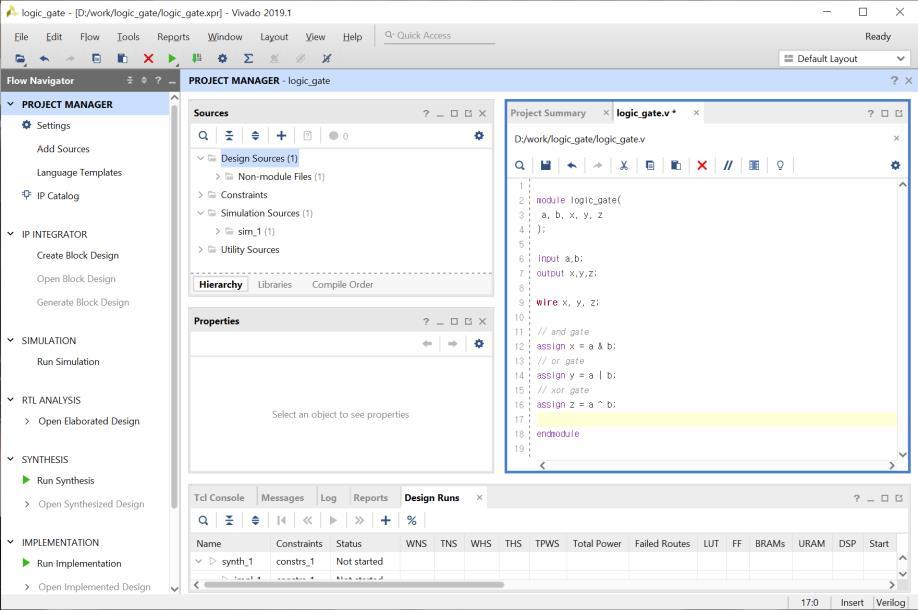
\includegraphics[width=\textwidth,height=4.6cm,keepaspectratio]{assets/legacy-01/p014-01.jpg}
\par}
\legacySource{14}
\end{frame}

\begin{frame}{로직 설계 및 합성}
\small
{\color{UOSBlue}\bfseries (2) 로직 설계}\par\vspace{0.12cm}
\begin{itemize}
\setlength{\itemsep}{0.08cm}
\item {로직 설계}
\end{itemize}
\par\vspace{0.12cm}
{\centering
\includegraphics[width=\textwidth,height=4.6cm,keepaspectratio]{assets/legacy-01/p014-02.png}
\par}
\legacySource{14}
\end{frame}

\begin{frame}[label=legacy-01-p15]{로직 설계 및 합성}
\small
{\color{UOSBlue}\bfseries (2) 로직 설계}\par\vspace{0.12cm}
\begin{itemize}
\setlength{\itemsep}{0.08cm}
\item {PROJECT MANAGER \textgreater{} Add Sources 선택}
\end{itemize}
\par\vspace{0.12cm}
{\centering
\includegraphics[width=\textwidth,height=4.6cm,keepaspectratio]{assets/legacy-01/p015-01.png}
\par}
\legacySource{15}
\end{frame}

\begin{frame}[label=legacy-01-p16]{로직 설계 및 합성}
\small
{\color{UOSBlue}\bfseries (2) 로직 설계}\par\vspace{0.12cm}
\begin{itemize}
\setlength{\itemsep}{0.08cm}
\item {Add Sources 창에서 Add or Create design sources 선택}
\end{itemize}
\par\vspace{0.12cm}
{\centering
\includegraphics[width=\textwidth,height=4.6cm,keepaspectratio]{assets/legacy-01/p016-01.png}
\par}
\legacySource{16}
\end{frame}

\begin{frame}[label=legacy-01-p17]{로직 설계 및 합성}
\small
{\color{UOSBlue}\bfseries (2) 로직 설계}\par\vspace{0.12cm}
\begin{itemize}
\setlength{\itemsep}{0.08cm}
\item {Add Files 버튼을 눌러, 앞의 logic\_gate.v 파일 추가}
\end{itemize}
\par\vspace{0.12cm}
{\centering
\includegraphics[width=\textwidth,height=4.6cm,keepaspectratio]{assets/legacy-01/p017-01.png}
\par}
\legacySource{17}
\end{frame}

\begin{frame}{로직 설계 및 합성}
\small
{\color{UOSBlue}\bfseries (2) 로직 설계}\par\vspace{0.12cm}
\begin{itemize}
\setlength{\itemsep}{0.08cm}
\item {Add Files 버튼을 눌러, 앞의 logic\_gate.v 파일 추가}
\end{itemize}
\par\vspace{0.12cm}
{\centering
\includegraphics[width=\textwidth,height=4.6cm,keepaspectratio]{assets/legacy-01/p017-02.png}
\par}
\legacySource{17}
\end{frame}

\begin{frame}[label=legacy-01-p18]{로직 설계 및 합성}
\small
{\color{UOSBlue}\bfseries (2) 로직 설계}\par\vspace{0.12cm}
\begin{itemize}
\setlength{\itemsep}{0.08cm}
\item {Sources 창에서 파일 추가된 것을 확인}
\end{itemize}
\par\vspace{0.12cm}
{\centering
\includegraphics[width=\textwidth,height=4.6cm,keepaspectratio]{assets/legacy-01/p018-01.png}
\par}
\legacySource{18}
\end{frame}

\begin{frame}[label=legacy-01-p19]{로직 설계 및 합성}
\small
{\color{UOSBlue}\bfseries (3) Assignment}\par\vspace{0.12cm}
\begin{itemize}
\setlength{\itemsep}{0.08cm}
\item {프로젝트의 타겟이 되는 FPGA 디바이스와 설계된 로직에서 사용하는 입출력 단자를 하드웨어와 연결하기 위하여 핀을 설정하는 것}
\end{itemize}
\legacySource{19}
\end{frame}

\begin{frame}[label=legacy-01-p20]{로직 설계 및 합성}
\small
{\color{UOSBlue}\bfseries (3) Assignment}\par\vspace{0.12cm}
\begin{itemize}
\setlength{\itemsep}{0.08cm}
\item {PROJECT MANAGER의 RTL ANALYSIS 탭의 Open Elaborated Design 부분을 마우스로 클릭}
\end{itemize}
\par\vspace{0.12cm}
{\centering
\includegraphics[width=\textwidth,height=4.6cm,keepaspectratio]{assets/legacy-01/p020-01.png}
\par}
\legacySource{20}
\end{frame}

\begin{frame}[label=legacy-01-p21]{로직 설계 및 합성}
\small
{\color{UOSBlue}\bfseries (3) Assignment}\par\vspace{0.12cm}
\begin{itemize}
\setlength{\itemsep}{0.08cm}
\item {메시지 창이 나타난다.}
\item {OK 버튼을 누르면 Elaboration 과정이 진행됨.}
\item {문법에 오류부분도 같이 체크하여 오류가 있다면 에러 메시지가 출력됨.}
\end{itemize}
\legacySource{21}
\end{frame}

\begin{frame}{로직 설계 및 합성}
\small
{\color{UOSBlue}\bfseries (3) Assignment}\par\vspace{0.12cm}
{\scriptsize 원문 설명에 대응하는 실제 화면}\par
\par\vspace{0.12cm}
{\centering
\includegraphics[width=\textwidth,height=4.6cm,keepaspectratio]{assets/legacy-01/p021-01.png}
\par}
\legacySource{21}
\end{frame}

\begin{frame}[label=legacy-01-p22]{로직 설계 및 합성}
\small
{\color{UOSBlue}\bfseries (3) Assignment}\par\vspace{0.12cm}
\begin{itemize}
\setlength{\itemsep}{0.08cm}
\item {설계된 Verilog HDL 구문이 Schematic으로 표현되는 것을 확인}
\end{itemize}
\par\vspace{0.12cm}
{\centering
\includegraphics[width=\textwidth,height=4.6cm,keepaspectratio]{assets/legacy-01/p022-01.png}
\par}
\legacySource{22}
\end{frame}

\begin{frame}[label=legacy-01-p23]{로직 설계 및 합성}
\small
{\color{UOSBlue}\bfseries (3) Assignment}\par\vspace{0.12cm}
\begin{itemize}
\setlength{\itemsep}{0.08cm}
\item {Schematic 화면 오른 쪽 윗 부분의 5 I/O Ports 선택}
\end{itemize}
\par\vspace{0.12cm}
{\centering
\includegraphics[width=\textwidth,height=4.6cm,keepaspectratio]{assets/legacy-01/p023-01.png}
\par}
\legacySource{23}
\end{frame}

\begin{frame}[label=legacy-01-p24]{로직 설계 및 합성}
\small
{\color{UOSBlue}\bfseries (3) Assignment}\par\vspace{0.15cm}\begin{itemize}
\setlength{\itemsep}{0.08cm}
\item {I/O Std를 “LVCMOSS33” 으로 변경}
\item {입/출력 포트의 Voltage Level을 3.3V로 설정하는 것.}
\end{itemize}
\vspace{0.5cm}\centering
\renewcommand{\arraystretch}{1.45}
\begin{tabular}{ccc|ccc}
포트 이름 & 핀 번호 & & 포트 이름 & 핀 번호 &\\\hline
\texttt{a} & K4 & SW\_1 & \texttt{x} & L4 & LED1\\
\texttt{b} & N8 & SW\_2 & \texttt{y} & M4 & LED2\\
& & & \texttt{z} & M2 & LED3
\end{tabular}
\par\vspace{0.4cm}
{\scriptsize 원문 표기 유지. 실제 속성값은 \navlink{legacy-01-notes}{보충 설명}을 확인한다.}

\legacySource{24}
\end{frame}

\begin{frame}[label=legacy-01-p25]{로직 설계 및 합성}
\small
{\color{UOSBlue}\bfseries (3) Assignment}\par\vspace{0.12cm}
\begin{itemize}
\setlength{\itemsep}{0.08cm}
\item {Package Pin 부분에 핀 설정}
\item {I/O Std를 “LVCMOSS33” 으로 변경}
\item {입/출력 포트의 Voltage Level을 3.3V로 설정하는 것.}
\end{itemize}
\legacySource{25}
\end{frame}

\begin{frame}{로직 설계 및 합성}
\small
{\color{UOSBlue}\bfseries (3) Assignment}\par\vspace{0.12cm}
{\scriptsize 원문 설명에 대응하는 실제 화면}\par
\par\vspace{0.12cm}
{\centering
\includegraphics[width=\textwidth,height=4.6cm,keepaspectratio]{assets/legacy-01/p025-01.png}
\par}
\legacySource{25}
\end{frame}

\begin{frame}[label=legacy-01-p26]{로직 설계 및 합성}
\small
{\color{UOSBlue}\bfseries (3) Assignment}\par\vspace{0.12cm}
\begin{itemize}
\setlength{\itemsep}{0.08cm}
\item {핀 설정 저장}
\item {파일 명은 logic\_gate로 설정}
\end{itemize}
\par\vspace{0.12cm}
{\centering
\includegraphics[width=\textwidth,height=4.15cm,keepaspectratio]{assets/legacy-01/p026-01.png}
\par}
\legacySource{26}
\end{frame}

\begin{frame}{로직 설계 및 합성}
\small
{\color{UOSBlue}\bfseries (3) Assignment}\par\vspace{0.12cm}
\begin{itemize}
\setlength{\itemsep}{0.08cm}
\item {핀 설정 저장}
\item {파일 명은 logic\_gate로 설정}
\end{itemize}
\par\vspace{0.12cm}
{\centering
\includegraphics[width=\textwidth,height=4.15cm,keepaspectratio]{assets/legacy-01/p026-02.png}
\par}
\legacySource{26}
\end{frame}

\begin{frame}[label=legacy-01-p27]{로직 설계 및 합성}
\small
{\color{UOSBlue}\bfseries (3) Assignment}\par\vspace{0.12cm}
\begin{itemize}
\setlength{\itemsep}{0.08cm}
\item {Sources 창에 추가된 것 확인}
\end{itemize}
\par\vspace{0.12cm}
{\centering
\includegraphics[width=\textwidth,height=4.6cm,keepaspectratio]{assets/legacy-01/p027-01.png}
\par}
\legacySource{27}
\end{frame}

\begin{frame}[label=legacy-01-p28]{로직 설계 및 합성}
\small
{\color{UOSBlue}\bfseries (4) Compile}\par\vspace{0.12cm}
\begin{itemize}
\setlength{\itemsep}{0.08cm}
\item {SYNTHESIS \textgreater{} Run Synthesis}
\item {설계된 Verilog HDL 코드를 합성하여 최적화 시키는 과정}
\end{itemize}
\par\vspace{0.12cm}
{\centering
\includegraphics[width=\textwidth,height=4.15cm,keepaspectratio]{assets/legacy-01/p028-01.png}
\par}
\legacySource{28}
\end{frame}

\begin{frame}{로직 설계 및 합성}
\small
{\color{UOSBlue}\bfseries (4) Compile}\par\vspace{0.12cm}
\begin{itemize}
\setlength{\itemsep}{0.08cm}
\item {SYNTHESIS \textgreater{} Run Synthesis}
\item {설계된 Verilog HDL 코드를 합성하여 최적화 시키는 과정}
\end{itemize}
\par\vspace{0.12cm}
{\centering
\includegraphics[width=\textwidth,height=4.15cm,keepaspectratio]{assets/legacy-01/p028-02.png}
\par}
\legacySource{28}
\end{frame}

\begin{frame}[label=legacy-01-p29]{로직 설계 및 합성}
\small
{\color{UOSBlue}\bfseries (4) Compile}\par\vspace{0.12cm}
\begin{itemize}
\setlength{\itemsep}{0.08cm}
\item {Synthesis 동작 확인 위치}
\item {프로그램 상단 오른쪽 회전}
\end{itemize}
\par\vspace{0.12cm}
{\centering
\includegraphics[width=\textwidth,height=4.15cm,keepaspectratio]{assets/legacy-01/p029-01.png}
\par}
\legacySource{29}
\end{frame}

\begin{frame}[label=legacy-01-p30]{로직 설계 및 합성}
\small
{\color{UOSBlue}\bfseries (4) Compile}\par\vspace{0.12cm}
\begin{itemize}
\setlength{\itemsep}{0.08cm}
\item {Synthesis 후 IMPLEMENTATION 진행}
\item {Implementation}
\item {합성한 결과를 이용하여 실제 FPGA의 Logic Cell 단위로 바꾸어 FPGA내에 위치시키고 연결하는 Place \& Route를 하는 과정}
\end{itemize}
\legacySource{30}
\end{frame}

\begin{frame}{로직 설계 및 합성}
\small
{\color{UOSBlue}\bfseries (4) Compile}\par\vspace{0.12cm}
{\scriptsize 원문 설명에 대응하는 실제 화면}\par
\par\vspace{0.12cm}
{\centering
\includegraphics[width=\textwidth,height=4.6cm,keepaspectratio]{assets/legacy-01/p030-01.png}
\par}
\legacySource{30}
\end{frame}

\begin{frame}{로직 설계 및 합성}
\small
{\color{UOSBlue}\bfseries (4) Compile}\par\vspace{0.12cm}
{\scriptsize 원문 설명에 대응하는 실제 화면}\par
\par\vspace{0.12cm}
{\centering
\includegraphics[width=\textwidth,height=4.6cm,keepaspectratio]{assets/legacy-01/p030-02.png}
\par}
\legacySource{30}
\end{frame}

\begin{frame}[label=legacy-01-p31]{로직 설계 및 합성}
\small
{\color{UOSBlue}\bfseries (4) Compile}\par\vspace{0.12cm}
\begin{itemize}
\setlength{\itemsep}{0.08cm}
\item {Synthesis 후 IMPLEMENTATION 진행}
\end{itemize}
\par\vspace{0.12cm}
{\centering
\includegraphics[width=\textwidth,height=4.6cm,keepaspectratio]{assets/legacy-01/p031-01.png}
\par}
\legacySource{31}
\end{frame}

\begin{frame}{로직 설계 및 합성}
\small
{\color{UOSBlue}\bfseries (4) Compile}\par\vspace{0.12cm}
\begin{itemize}
\setlength{\itemsep}{0.08cm}
\item {Synthesis 후 IMPLEMENTATION 진행}
\end{itemize}
\par\vspace{0.12cm}
{\centering
\includegraphics[width=\textwidth,height=4.6cm,keepaspectratio]{assets/legacy-01/p031-02.png}
\par}
\legacySource{31}
\end{frame}

\begin{frame}[label=legacy-01-p32]{로직 설계 및 합성}
\small
{\color{UOSBlue}\bfseries (4) Compile}\par\vspace{0.12cm}
\begin{itemize}
\setlength{\itemsep}{0.08cm}
\item {Implementation 이 끝난 화면}
\item {Open Implemented Design 선택 후 OK}
\end{itemize}
\par\vspace{0.12cm}
{\centering
\includegraphics[width=\textwidth,height=4.15cm,keepaspectratio]{assets/legacy-01/p032-01.png}
\par}
\legacySource{32}
\end{frame}

\begin{frame}[label=legacy-01-p33]{로직 설계 및 합성}
\small
{\color{UOSBlue}\bfseries (4) Compile}\par\vspace{0.12cm}
\begin{itemize}
\setlength{\itemsep}{0.08cm}
\item {Implementation결과 확인}
\end{itemize}
\par\vspace{0.12cm}
{\centering
\includegraphics[width=\textwidth,height=4.6cm,keepaspectratio]{assets/legacy-01/p033-01.png}
\par}
\legacySource{33}
\end{frame}

\begin{frame}[label=legacy-01-p34]{로직 설계 및 합성}
\small
{\color{UOSBlue}\bfseries (5) Simulation}\par\vspace{0.12cm}
\begin{itemize}
\setlength{\itemsep}{0.08cm}
\item {소프트웨어적으로 검증하는 과정}
\item {테스트 벤치 파일이 필요함.}
\item {시뮬레이션에 대한 입력 조건을 설정한 파일}
\end{itemize}
\legacySource{34}
\end{frame}

\begin{frame}[label=legacy-01-p35]{로직 설계 및 합성}
\small
{\color{UOSBlue}\bfseries (5) Simulation}\par\vspace{0.12cm}
\begin{itemize}
\setlength{\itemsep}{0.08cm}
\item {File \textgreater{} Text Editor \textgreater{} New File 선택}
\end{itemize}
\par\vspace{0.12cm}
{\centering
\includegraphics[width=\textwidth,height=4.6cm,keepaspectratio]{assets/legacy-01/p035-01.png}
\par}
\legacySource{35}
\end{frame}

\begin{frame}[label=legacy-01-p36]{로직 설계 및 합성}
\small
{\color{UOSBlue}\bfseries (5) Simulation}\par\vspace{0.12cm}
\begin{itemize}
\setlength{\itemsep}{0.08cm}
\item {testbench.v 파일로 저장}
\end{itemize}
\par\vspace{0.12cm}
{\centering
\includegraphics[width=\textwidth,height=4.6cm,keepaspectratio]{assets/legacy-01/p036-01.png}
\par}
\legacySource{36}
\end{frame}

\begin{frame}[label=legacy-01-p37]{로직 설계 및 합성}
\small
{\color{UOSBlue}\bfseries (5) Simulation}\par\vspace{0.12cm}
\begin{itemize}
\setlength{\itemsep}{0.08cm}
\item {PROJECT MANAGER Add Source 선택}
\end{itemize}
\par\vspace{0.12cm}
{\centering
\includegraphics[width=\textwidth,height=4.6cm,keepaspectratio]{assets/legacy-01/p037-01.png}
\par}
\legacySource{37}
\end{frame}

\begin{frame}[label=legacy-01-p38]{로직 설계 및 합성}
\small
{\color{UOSBlue}\bfseries (5) Simulation}\par\vspace{0.12cm}
\begin{itemize}
\setlength{\itemsep}{0.08cm}
\item {[Add or create simulation source] 선택}
\item {Next}
\end{itemize}
\par\vspace{0.12cm}
{\centering
\includegraphics[width=\textwidth,height=4.15cm,keepaspectratio]{assets/legacy-01/p038-01.png}
\par}
\legacySource{38}
\end{frame}

\begin{frame}[label=legacy-01-p39]{로직 설계 및 합성}
\small
{\color{UOSBlue}\bfseries (5) Simulation}\par\vspace{0.12cm}
\begin{itemize}
\setlength{\itemsep}{0.08cm}
\item {[Add Files]을 선택}
\item {testbench.v 파일 선택}
\end{itemize}
\par\vspace{0.12cm}
{\centering
\includegraphics[width=\textwidth,height=4.15cm,keepaspectratio]{assets/legacy-01/p039-01.png}
\par}
\legacySource{39}
\end{frame}

\begin{frame}{로직 설계 및 합성}
\small
{\color{UOSBlue}\bfseries (5) Simulation}\par\vspace{0.12cm}
\begin{itemize}
\setlength{\itemsep}{0.08cm}
\item {[Add Files]을 선택}
\item {testbench.v 파일 선택}
\end{itemize}
\par\vspace{0.12cm}
{\centering
\includegraphics[width=\textwidth,height=4.15cm,keepaspectratio]{assets/legacy-01/p039-02.png}
\par}
\legacySource{39}
\end{frame}

\begin{frame}[label=legacy-01-p40]{로직 설계 및 합성}
\small
{\color{UOSBlue}\bfseries (5) Simulation}\par\vspace{0.12cm}
\begin{itemize}
\setlength{\itemsep}{0.08cm}
\item {Simulation Sources 파일 추가 확인}
\end{itemize}
\par\vspace{0.12cm}
{\centering
\includegraphics[width=\textwidth,height=4.6cm,keepaspectratio]{assets/legacy-01/p040-01.png}
\par}
\legacySource{40}
\end{frame}

\begin{frame}[label=legacy-01-p41]{로직 설계 및 합성}
\small
{\color{UOSBlue}\bfseries (5) Simulation}\par\vspace{0.12cm}
\begin{itemize}
\setlength{\itemsep}{0.08cm}
\item {SIMULATION \textgreater{} Run Simulation}
\item {Run Behavioral Simulation 실행}
\end{itemize}
\par\vspace{0.12cm}
{\centering
\includegraphics[width=\textwidth,height=4.15cm,keepaspectratio]{assets/legacy-01/p041-01.png}
\par}
\legacySource{41}
\end{frame}

\begin{frame}[label=legacy-01-p42]{로직 설계 및 합성}
\small
{\color{UOSBlue}\bfseries (5) Simulation}\par\vspace{0.12cm}
\begin{itemize}
\setlength{\itemsep}{0.08cm}
\item {결과 확인}
\item {상단 우측의 Maximize 버튼 클릭}
\end{itemize}
\par\vspace{0.12cm}
{\centering
\includegraphics[width=\textwidth,height=4.15cm,keepaspectratio]{assets/legacy-01/p042-01.png}
\par}
\legacySource{42}
\end{frame}

\begin{frame}[label=legacy-01-p43]{로직 설계 및 합성}
\small
{\color{UOSBlue}\bfseries (5) Simulation}\par\vspace{0.12cm}
\begin{itemize}
\setlength{\itemsep}{0.08cm}
\item {Zoom Fit 를 눌러 결과 확인}
\end{itemize}
\par\vspace{0.12cm}
{\centering
\includegraphics[width=\textwidth,height=4.6cm,keepaspectratio]{assets/legacy-01/p043-01.png}
\par}
\legacySource{43}
\end{frame}

\begin{frame}[label=legacy-01-p44]{로직 설계 및 합성}
\small
{\color{UOSBlue}\bfseries (6) Programming}\par\vspace{0.12cm}
\begin{itemize}
\setlength{\itemsep}{0.08cm}
\item {Project Manager 창 PROGRAM AND DEBUG \textgreater{} Generate Bitstream}
\end{itemize}
\par\vspace{0.12cm}
{\centering
\includegraphics[width=\textwidth,height=4.6cm,keepaspectratio]{assets/legacy-01/p044-01.png}
\par}
\legacySource{44}
\end{frame}

\begin{frame}{로직 설계 및 합성}
\small
{\color{UOSBlue}\bfseries (6) Programming}\par\vspace{0.12cm}
\begin{itemize}
\setlength{\itemsep}{0.08cm}
\item {Project Manager 창 PROGRAM AND DEBUG \textgreater{} Generate Bitstream}
\end{itemize}
\par\vspace{0.12cm}
{\centering
\includegraphics[width=\textwidth,height=4.6cm,keepaspectratio]{assets/legacy-01/p044-02.png}
\par}
\legacySource{44}
\end{frame}

\begin{frame}[label=legacy-01-p45]{로직 설계 및 합성}
\small
{\color{UOSBlue}\bfseries (6) Programming}\par\vspace{0.12cm}
\begin{itemize}
\setlength{\itemsep}{0.08cm}
\item {프로그래밍 파일 생성 완료 후}
\item {Open Hardware Manager}
\end{itemize}
\par\vspace{0.12cm}
{\centering
\includegraphics[width=\textwidth,height=4.15cm,keepaspectratio]{assets/legacy-01/p045-01.png}
\par}
\legacySource{45}
\end{frame}

\begin{frame}[label=legacy-01-p46]{로직 설계 및 합성}
\small
{\color{UOSBlue}\bfseries (6) Programming}\par\vspace{0.12cm}
\begin{itemize}
\setlength{\itemsep}{0.08cm}
\item {하드웨어 준비}
\end{itemize}
\par\vspace{0.12cm}
{\centering
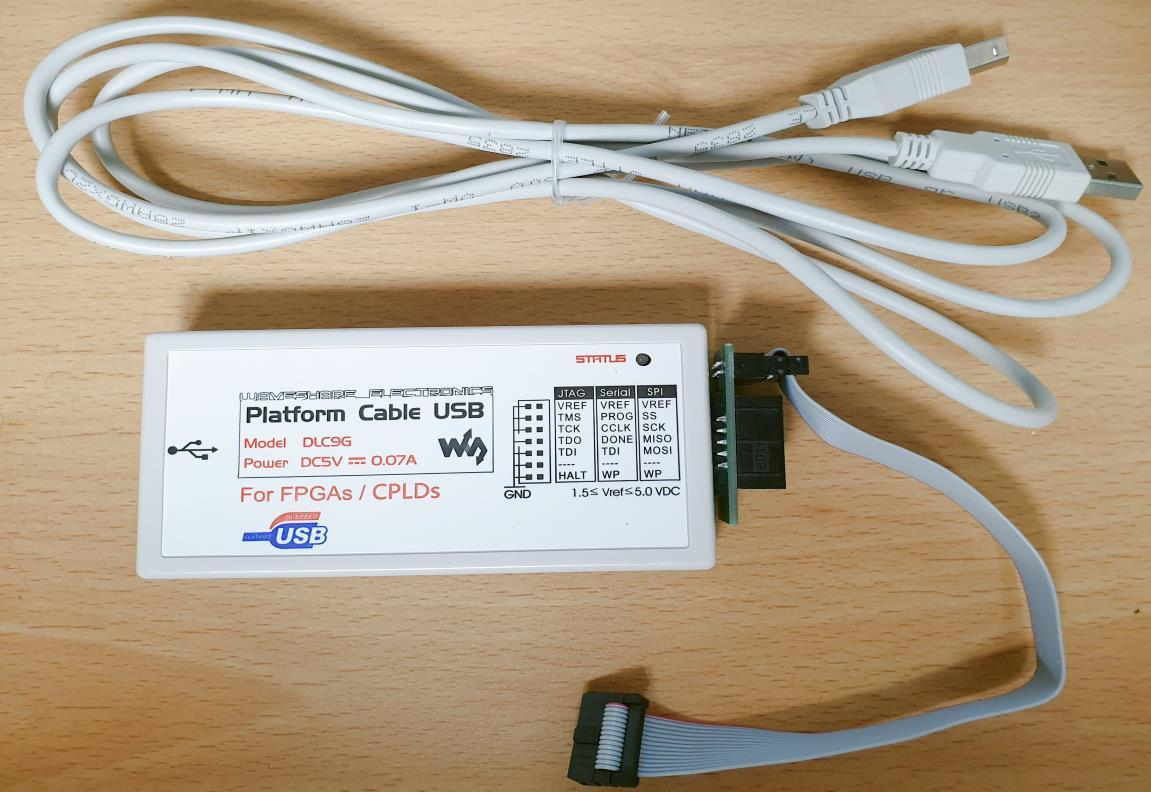
\includegraphics[width=\textwidth,height=4.6cm,keepaspectratio]{assets/legacy-01/p046-01.jpg}
\par}
\legacySource{46}
\end{frame}

\begin{frame}[label=legacy-01-p47]{로직 설계 및 합성}
\small
{\color{UOSBlue}\bfseries (6) Programming}\par\vspace{0.12cm}
\begin{itemize}
\setlength{\itemsep}{0.08cm}
\item {장비의 전원이 꺼져 있는지 확인}
\item {Xilinx Platform Cable에 USB Cable의 한 쪽 끝을 연결}
\item {반대쪽 끝은 PC의 USB 포트에 연결}
\item {Xilinx Platform Cable에 연결된 2x14핀의 플랫 케이블은 장비의 Xilinx 모듈의 JTAG 포트에 연결}
\item {장비의 전원을 켠다.}
\end{itemize}
\legacySource{47}
\end{frame}

\begin{frame}[label=legacy-01-p48]{로직 설계 및 합성}
\small
{\color{UOSBlue}\bfseries (6) Programming}\par\vspace{0.12cm}
\begin{itemize}
\setlength{\itemsep}{0.08cm}
\item {Xilinx Platform II Cable을 PC에 연결한 후, PC의 장치관리자에서 장치 인식 확인}
\end{itemize}
\par\vspace{0.12cm}
{\centering
\includegraphics[width=\textwidth,height=4.6cm,keepaspectratio]{assets/legacy-01/p048-01.png}
\par}
\legacySource{48}
\end{frame}

\begin{frame}[label=legacy-01-p49]{로직 설계 및 합성}
\small
{\color{UOSBlue}\bfseries (6) Programming}\par\vspace{0.12cm}
\begin{itemize}
\setlength{\itemsep}{0.08cm}
\item {Open Target \textgreater{} Auto Connect}
\end{itemize}
\par\vspace{0.12cm}
{\centering
\includegraphics[width=\textwidth,height=4.6cm,keepaspectratio]{assets/legacy-01/p049-01.png}
\par}
\legacySource{49}
\end{frame}

\begin{frame}[label=legacy-01-p50]{로직 설계 및 합성}
\small
{\color{UOSBlue}\bfseries (6) Programming}\par\vspace{0.12cm}
\begin{itemize}
\setlength{\itemsep}{0.08cm}
\item {Program Device 선택}
\end{itemize}
\par\vspace{0.12cm}
{\centering
\includegraphics[width=\textwidth,height=4.6cm,keepaspectratio]{assets/legacy-01/p050-01.png}
\par}
\legacySource{50}
\end{frame}

\begin{frame}[label=legacy-01-p51]{로직 설계 및 합성}
\small
{\color{UOSBlue}\bfseries (6) Programming}\par\vspace{0.12cm}
\begin{itemize}
\setlength{\itemsep}{0.08cm}
\item {Bitstream File 선택}
\item {\textless{}Project Folder\textgreater{} \textbackslash{} logic\_gate.runs \textbackslash{} impl\_1 \textbackslash{} logic\_gate.bit 파일 선택}
\item {Program 버튼 클릭}
\end{itemize}
\legacySource{51}
\end{frame}

\begin{frame}{로직 설계 및 합성}
\small
{\color{UOSBlue}\bfseries (6) Programming}\par\vspace{0.12cm}
{\scriptsize 원문 설명에 대응하는 실제 화면}\par
\par\vspace{0.12cm}
{\centering
\includegraphics[width=\textwidth,height=4.6cm,keepaspectratio]{assets/legacy-01/p051-01.png}
\par}
\legacySource{51}
\end{frame}

\begin{frame}[label=legacy-01-p52]{로직 설계 및 합성}
\small
{\color{UOSBlue}\bfseries (7) 동작 확인}\par\vspace{0.12cm}
\begin{itemize}
\setlength{\itemsep}{0.08cm}
\item {SW 1와 SW 2를 눌러 장비에서 어떻게 동작하는지 확인.}
\end{itemize}
\legacySource{52}
\end{frame}

\begin{frame}[label=legacy-01-notes]{보충 · 원문 표기와 실행 조건}
\small

\begin{itemize}
\setlength{\itemsep}{0.3cm}
\item 원본 p.24--25의 \texttt{LVCMOSS33}은 오타다.\par
실제 I/O 표준은 \texttt{LVCMOS33}을 선택한다.
\item \texttt{d:/work}는 원본의 예시 작업 경로다.\par
실제 프로젝트를 저장한 경로를 사용한다.
\item 원본 테스트벤치는 10 ns 단위에서 \texttt{\#20}마다\par
입력을 바꾼다. 입력 전환 간격은 200 ns다.
\item 원본의 \texttt{a,b} 입력 순서는 00, 10, 01, 11이다.\par
출력 \texttt{x,y,z}를 AND·OR·XOR 진리표와 비교한다.
\end{itemize}
\vspace{0.3cm}
{\scriptsize 이 페이지는 원본과 구분한 보충 설명이다. 원본 코드 이미지는 유지했다.}

\end{frame}

\begin{frame}[label=legacy-01-prelab]{보충 · VS Code 사전 시뮬레이션}
\small

\begin{enumerate}
\setlength{\itemsep}{0.23cm}
\item \texttt{logic\_gate.v}와 테스트벤치를 VS Code에서 연다.
\item 배포 workspace의 02 Simulate로 자기검사 TB를 실행한다.
\item 원본 테스트벤치에는 자동 종료·VCD 저장 구문이 없다.\par
사전 실습은 별도 TB로 4개 입력·40 ns와 VCD를 검사한다.
\item 생성한 파형에서 \texttt{a,b,x,y,z}를 확인하고 예상값과 비교한다.
\item 실행 방법·코드 설명·파형 해석을 실험 전 레포트에 쓴다.
\end{enumerate}
\vspace{0.3cm}
{\scriptsize \href{02.vscode_verilog_환경설정_매뉴얼.pdf}{VS Code 환경설정 매뉴얼} ·
\navlink{lab1-reports}{레포트 안내}\par
사전 단계는 이번 수업의 보충 안내이며 원본 Vivado 화면과 구분한다.}

\end{frame}

\begin{frame}[label=legacy-01-postlab]{보충 · 보드 결과와 실험 후 레포트}
\small

\begin{enumerate}
\setlength{\itemsep}{0.22cm}
\item Vivado 파형을 VS Code 사전 시뮬레이션과 비교한다.
\item 생성한 \texttt{logic\_gate.bit}를 실제 FPGA에 기록한다.
\item SW\_1·SW\_2의 네 입력 조합과 LED1·LED2·LED3를 확인한다.
\item 연결 상태는 사진, 입력에 따른 출력 변화는 영상으로 남긴다.
\item 코드·파형·사진·영상을 GitHub에 올리고 레포트에 연결한다.
\end{enumerate}
\vspace{0.35cm}
실제 결과와 예상값을 비교하고 오류·수정 사항을 설명한다.\par
\vspace{0.2cm}
{\scriptsize 원본 화면의 성공 표시와 본인의 실행 결과를 구분한다.\par
\navlink{legacy-01-contents}{이 실습 목차} · \href{04.LAB1_00_CONTENTS.pdf}{전체 목차 PDF}}

\end{frame}


\begin{frame}[label=legacy-01-post]{실제 보드 연결}\relax
\small
\par\vspace{0.18cm}{\centering\includegraphics[width=\textwidth,height=3.0cm,keepaspectratio,trim=202.5bp 476.25bp 586.5bp 92.25bp,clip]{assets/modern-01/70-auto-connect.png}\par}\vspace{0.16cm}
Open Hardware Manager → Open target → Auto Connect.\par\vspace{0.22cm}KEY1=a, KEY2=b. LED1=x, LED2=y, LED3=z.\par\vspace{0.22cm}장치가 없으면 보드 전원·USB JTAG·드라이버·VM USB 연결을 점검한다.\par
\end{frame}

\begin{frame}{Program Device와 동작 확인}\relax
\small
\begin{enumerate}\setlength{\itemsep}{0.22cm}
\item 연결된 장치 이름이 xc7s75인지 확인한다.
\item 장치 우클릭 → Program Device.
\item 이번 프로젝트의 logic\_gate.bit를 선택하고 Program.
\item 기록 완료를 확인한 뒤 입력을 바꾸고 출력과 예상값을 비교한다.
\item 기록 성공 화면과 실제 보드 동작은 각각 증빙한다.
\end{enumerate}
제작 환경의 실제 보드 기록·촬영 검증 여부는 검증표를 따른다. 파일 생성만으로 보드 동작 성공을 선언하지 않는다.\par
\end{frame}

\begin{frame}{사진과 시연 영상 촬영}\relax
\small
KEY1=a, KEY2=b. LED1=x, LED2=y, LED3=z.\par\vspace{0.22cm}사진에는 보드 연결과 입력·출력 위치가 함께 보이게 한다.\par\vspace{0.22cm}영상에는 입력을 조작하는 과정과 그에 따른 출력 변화를 담는다.\par\vspace{0.22cm}예상표의 정상·경계 조건을 직접 보여주고 회로 번호를 파일명에 적는다.\par\vspace{0.22cm}통합 영상이라면 각 회로의 타임스탬프를 레포트에서 연결한다.\par
\end{frame}

\begin{frame}{GitHub 결과 정리}\relax
\small
\begin{enumerate}\setlength{\itemsep}{0.22cm}
\item reports/pre와 reports/post에 실험 전·후 레포트를 둔다.
\item evidence/vscode와 evidence/vivado에 로그·파형·캡처를 구분한다.
\item evidence/board/photos와 videos에 직접 촬영한 자료를 둔다.
\item 큰 영상·bit는 배포 위치를 정하고 README와 레포트에서 연결한다.
\item 웹에서 사진 표시와 영상 재생 또는 다운로드가 되는지 확인한다.
\end{enumerate}
\href{https://github.com/Glaysia/ece2_26_2_2/blob/daily/0910/example/fpga_projects_hdl/LAB1/docs/reports.md}{레포트 양식·예시·GitHub 안내}
\end{frame}

\begin{frame}{실험 후 레포트}\relax
\hypertarget{lab1-reports}{}\small
\begin{enumerate}\setlength{\itemsep}{0.22cm}
\item Vivado 버전·part·top·핀 제약·코드 커밋을 기록한다.
\item VS Code와 Vivado의 입력·출력·시간·검사 수를 비교한다.
\item 합성·구현·bit 경로와 경고·수정 사항을 설명한다.
\item 장치 기록 화면·사진·영상과 해당 조건을 연결한다.
\item 예상값·두 시뮬레이션·실측의 일치 또는 차이 원인을 해석한다.
\item 미수행 항목은 미완료로 남기고 후속 확인을 적는다.
\end{enumerate}
\href{04.LAB1_00_CONTENTS.pdf}{전체 목차 PDF}\quad\href{https://github.com/Glaysia/fpga-lab-example-legacy-01-logic-gates/tree/9055c8002ec5149907f393a1c781000d44125e38}{프로젝트로 돌아가기}
\end{frame}
\endgroup
\end{document}
